\part{Autonomous-ODEs}
\lecture{Autonomous ODEs}{Autonomous-ODEs}
\section{Autonomous ODEs}

\title{Ordinary Differential Equations}
\subtitle{Math 232 - Week 3, Day 2}
\date{11 September 2013}

\begin{frame}
  \titlepage
\end{frame}

\begin{frame}
  \frametitle{Outline}
  \tableofcontents[currentsection]

  Section 2.5 in book.
\end{frame}


\subsection{Solutions to DEs}


\begin{frame}
  \frametitle{What is a solution to a DE?}

  What is the solution to the DE

  \begin{eqnarray*}
    y' & = & t^2 + y^2?
  \end{eqnarray*}

  \uncover<2->{I do not know!}


\end{frame}


\begin{frame}
  \frametitle{Slope Field}

  Look at the slope field:
  \begin{eqnarray*}
    y' & = & t^2 + y^2?
  \end{eqnarray*}

  % TODO - make this image higher resolution!
  \only<1>{\includegraphics[height=5cm]{img/week3-D3SlopeExample}}
  \only<2->{\includegraphics[height=5cm]{img/week3-D3SlopeExampleSolutions}}

  Look at equilibria, stability, and look for straight line solutions.

\end{frame}


\iftoggle{clicker}{%
\begin{frame}
  \frametitle{Clicker Quiz}
    
      \ifnum\value{clickerQuiz}=1{%

        Look at the slope field:
        \begin{eqnarray*}
          y' & = & -t - y^2?
        \end{eqnarray*}

        \begin{columns}
          \column{.6\textwidth} 

          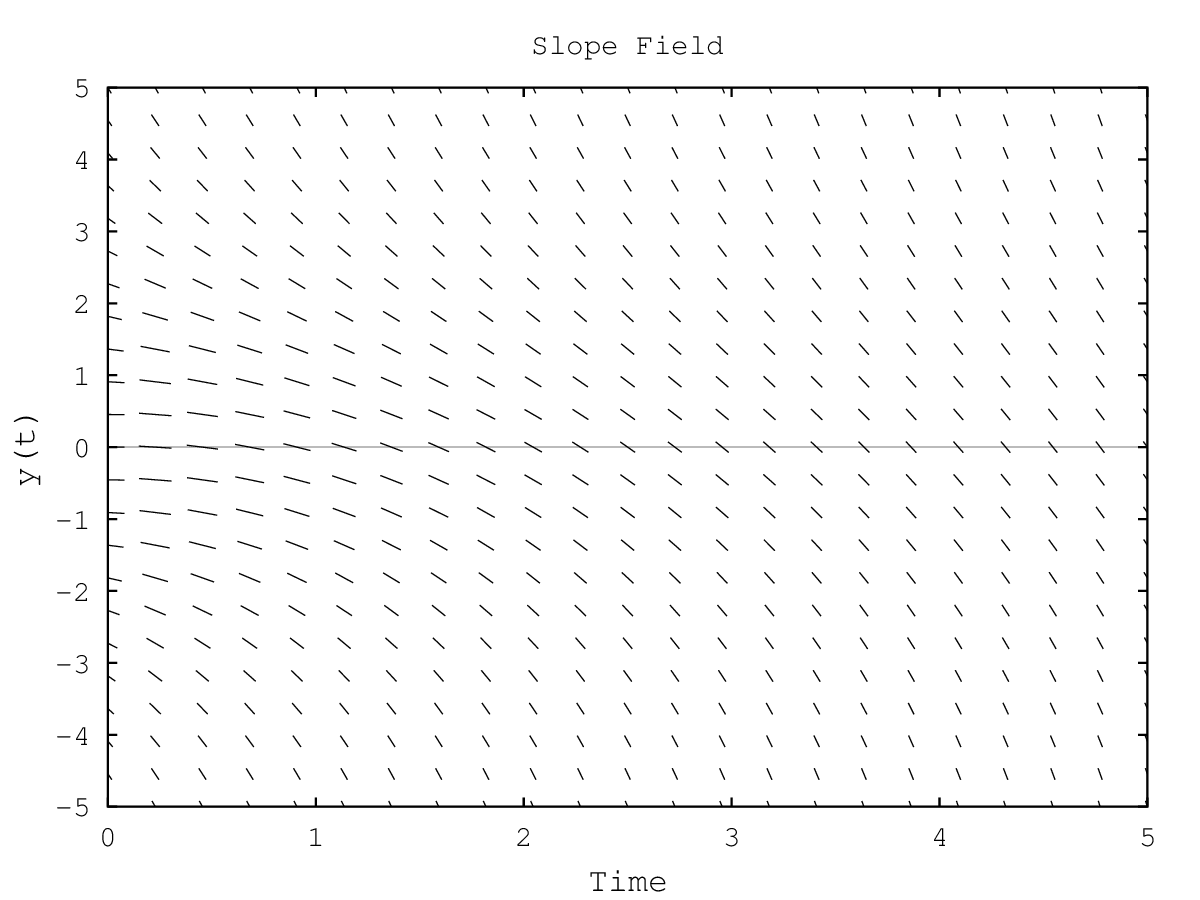
\includegraphics[height=5cm]{img/stabilityClicker1}

          \column{.4\textwidth}
          True or False: The solution to this differential equation is stable.

          \begin{tabular}{l@{\hspace{3em}}l}
            A: & True. \\
            B: & False. \\
            C: & Who knows? \\
            D: & Truth is subjective. \\ 
          \end{tabular}

        \end{columns}

     }\fi

     \ifnum\value{clickerQuiz}=2{%

        Look at the slope field:
        \begin{eqnarray*}
          y' & = & \frac{3}{2}-y?
        \end{eqnarray*}


        \begin{columns}
          \column{.6\textwidth} 

          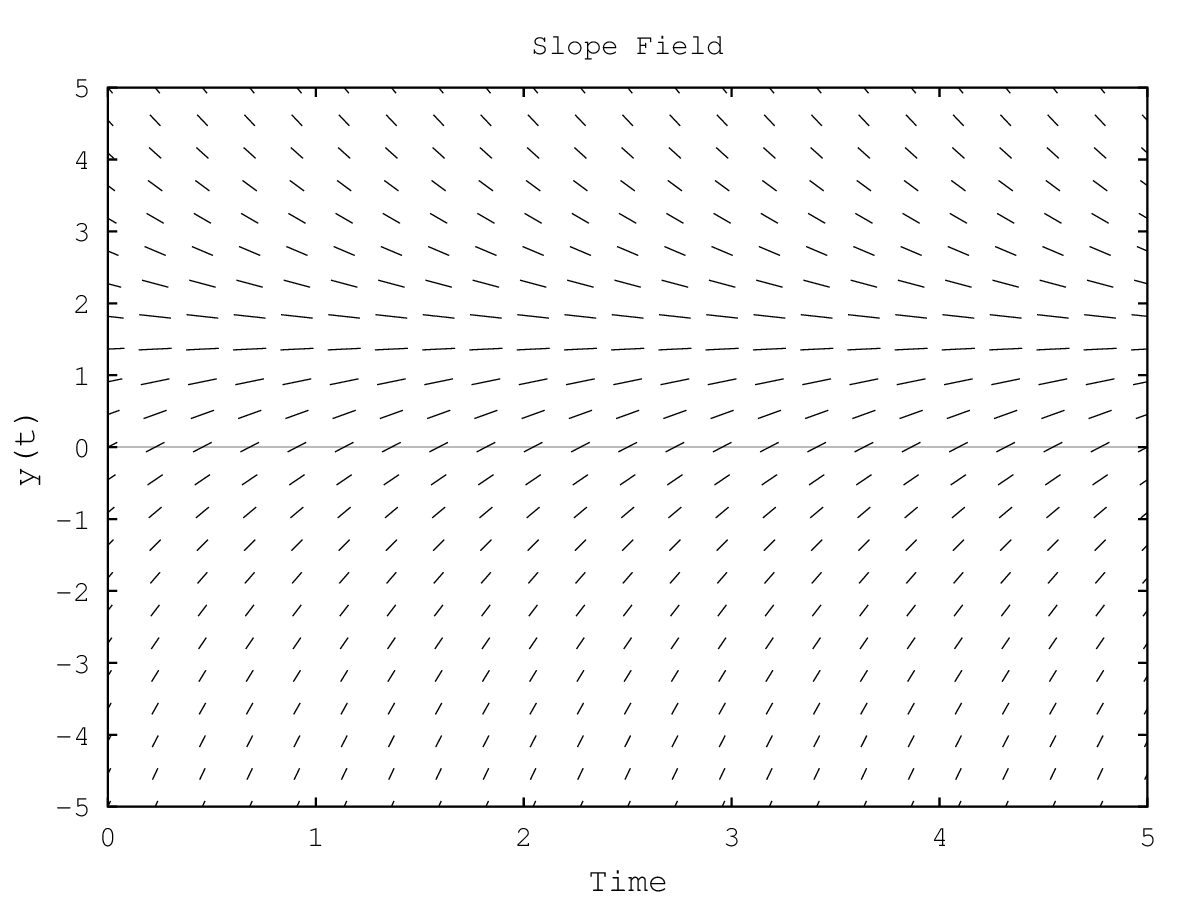
\includegraphics[height=5cm]{img/stabilityClicker2}

          \column{.4\textwidth}
          True or False: The solution to this differential equation is stable.

          \begin{tabular}{l@{\hspace{3em}}l}
            A: & True. \\
            B: & False. \\
            C: & Who knows? \\
            D: & Truth is subjective. \\ 
          \end{tabular}

        \end{columns}

     }\fi

      \ifnum\value{clickerQuiz}=3{%
        Given the slope field for the equation
        \begin{eqnarray*}
          x' & = & x^2-5?,
        \end{eqnarray*}
        determine if the equation is stable at $x=-\sqrt{5}$.


        \begin{columns}
          \column{.6\textwidth}

          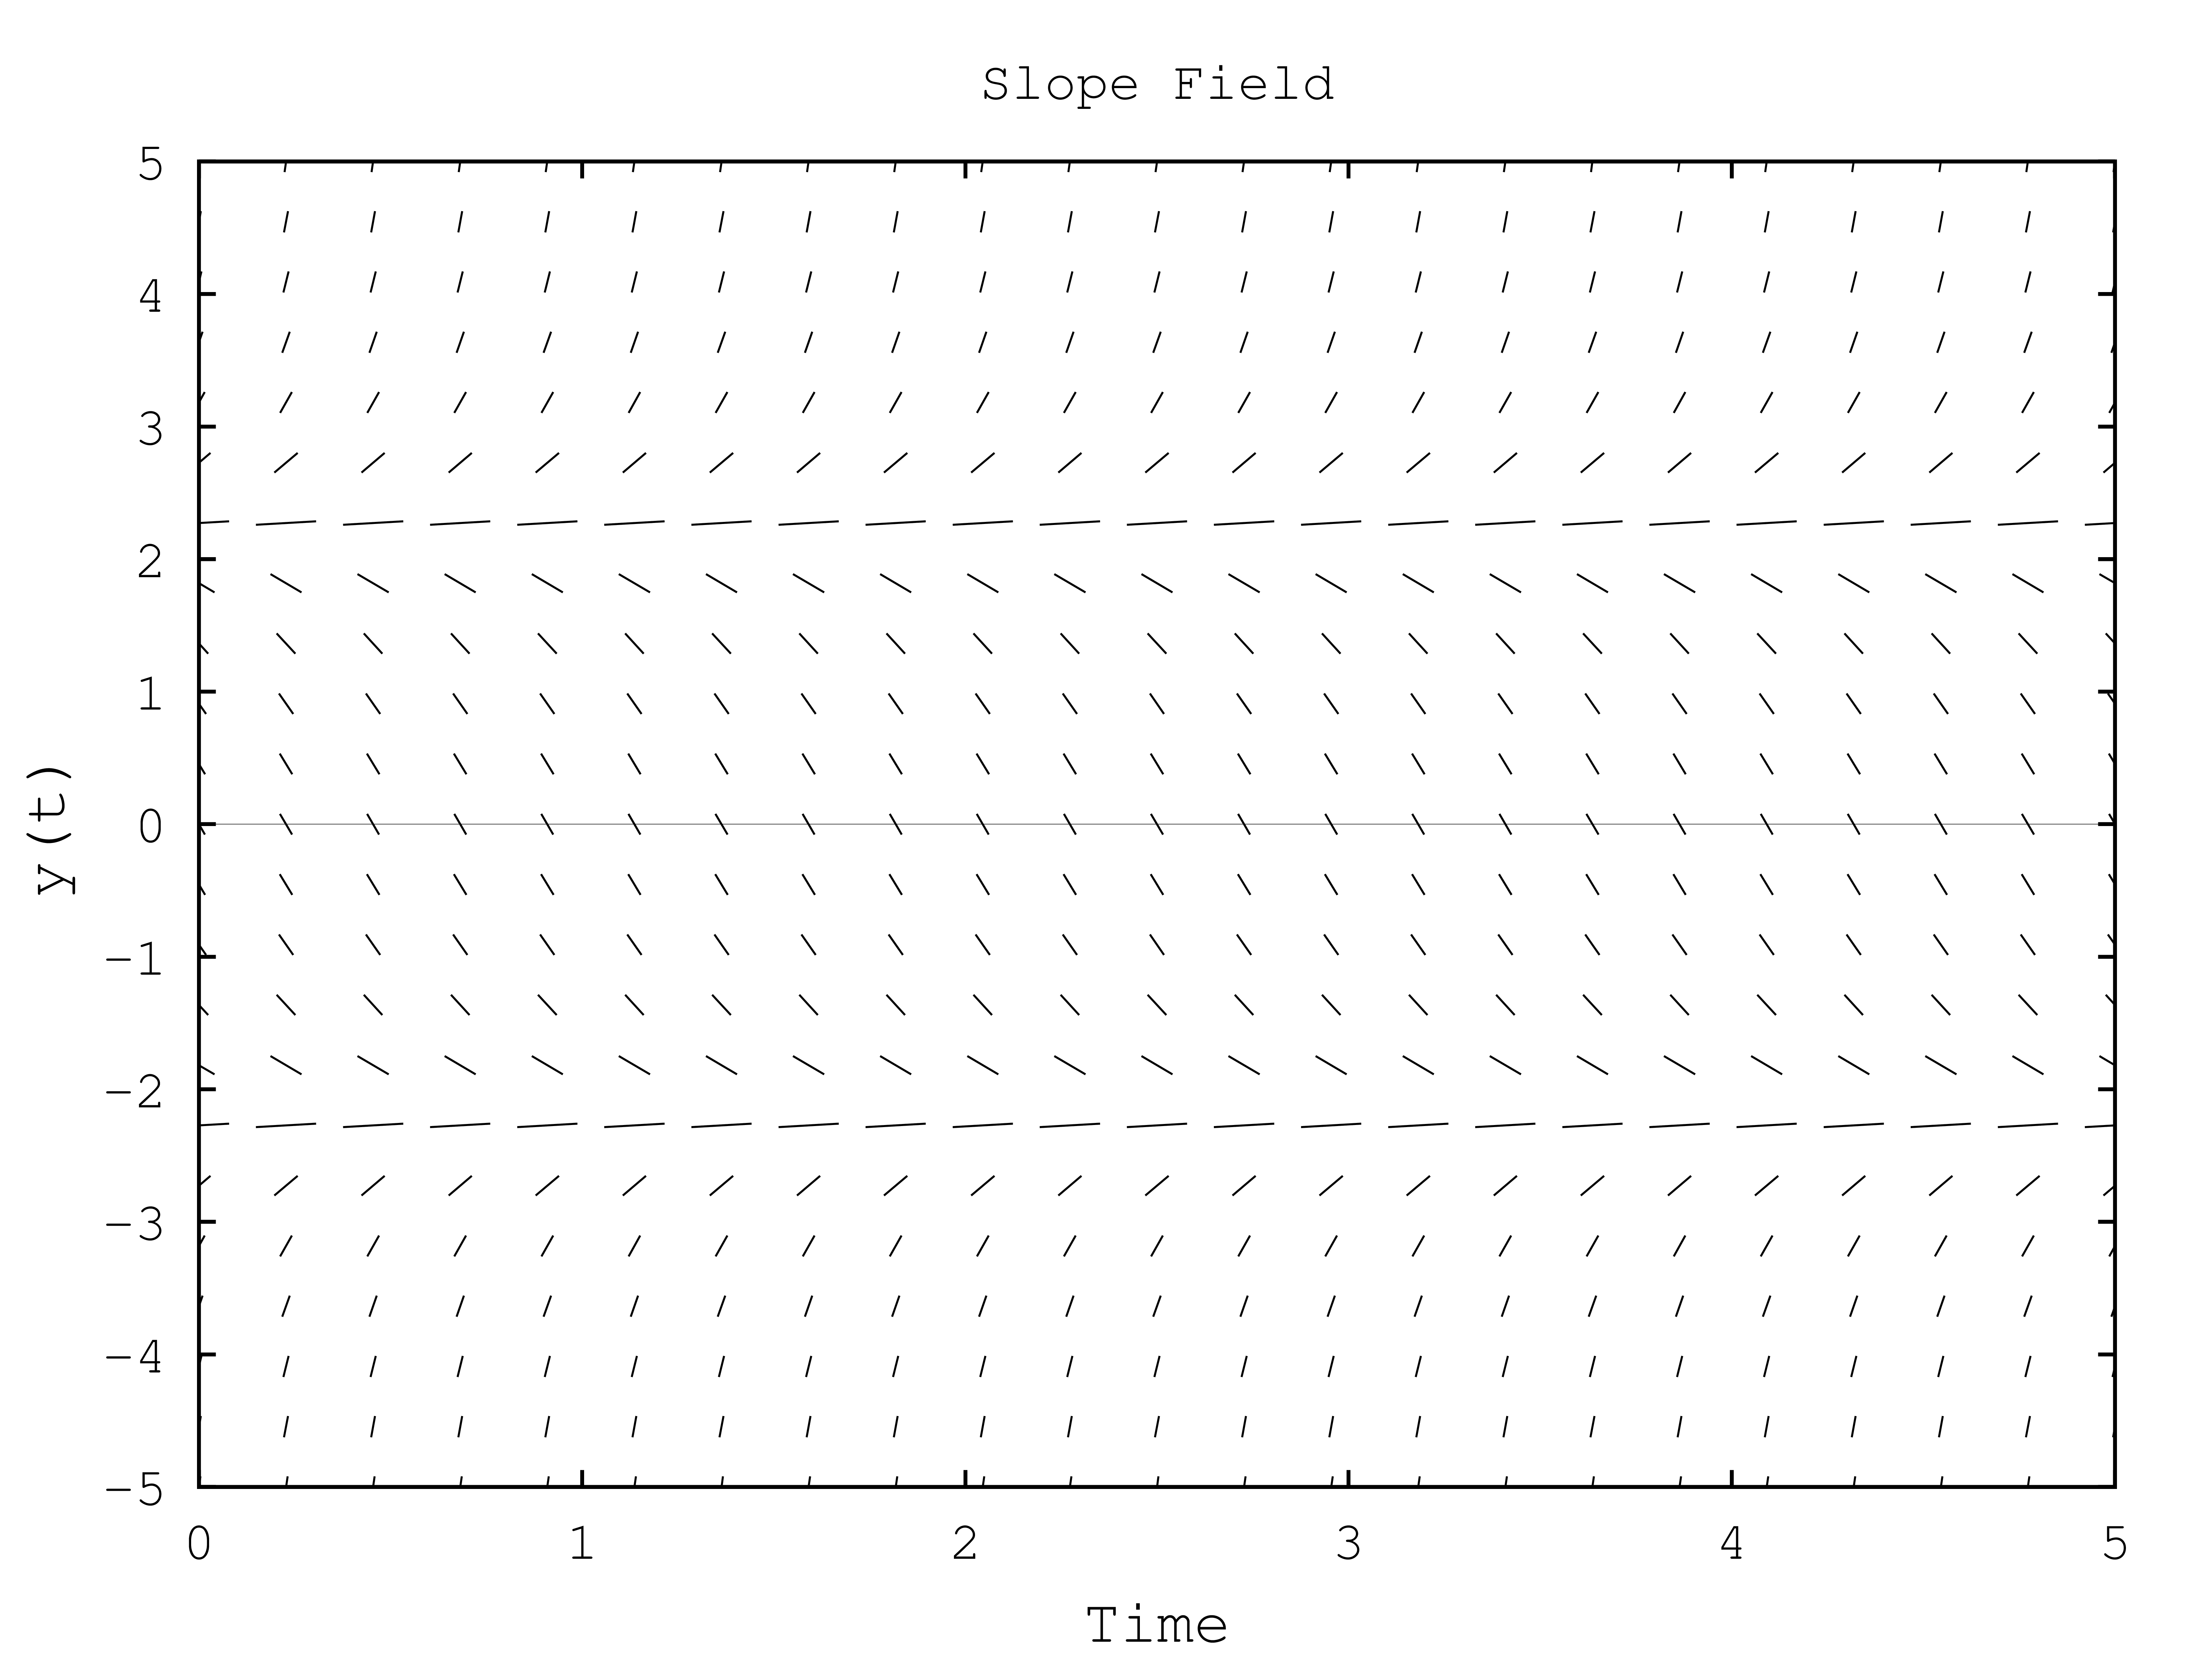
\includegraphics[height=5cm]{img/slopefield2}

          \column{.4\textwidth}
          True or False: The solution to this differential equation is stable.

          \begin{tabular}{l@{\hspace{1em}}l}
            A: & True. \\
            B: & False. \\
            C: & Who knows? \\
            D: & Truth is subjective. \\
          \end{tabular}

        \end{columns}

     }\fi

    \vfill
    \vfill
    \vfill

\end{frame}

}


\subsection{Autonomous DEs}

\begin{frame}
  \frametitle{Autonomous DEs}

  \begin{definition}
    A differential equation is \redText{\textit{autonomous}} if it can be
    expressed in the form
    \begin{eqnarray*}
      y' & = & f(y).
    \end{eqnarray*}
  \end{definition}
  i.e. the DE does not have a time term explicitly given in the
  equation.


\end{frame}


\begin{frame}{Example}
  
  \begin{columns}
    \column{.5\textwidth} 

    Autonomous:
    \begin{itemize}
    \item $y'=y$ 
    \item $y'=y^2+1$
    \item $y'=e^{-y}$.
    \end{itemize}

    \column{.5\textwidth} 

    Not Autonomous:
    \begin{itemize}
    \item $y'=y+t$ 
    \item $y'=\frac{y^2+1}{t}$
    \item $y'=e^{t-y}$.
    \end{itemize}

  \end{columns}

\end{frame}

\begin{frame}
  \frametitle{The slope only depends on y!}

  \vspace*{-3em}
  \begin{eqnarray*}
    y' & = & f(y).
  \end{eqnarray*}

  If the slope at $y=1$ and $t=1$ is $\half$, then it will be the same
  slope for all points where $y=1$. 

  \vfill
  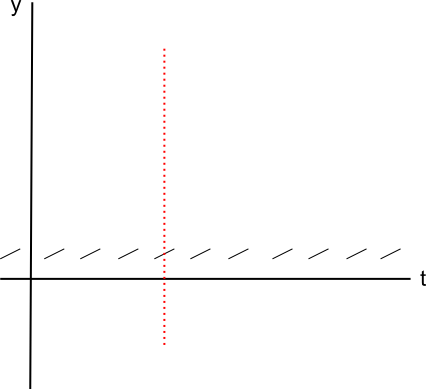
\includegraphics[width=5cm]{img/autonomousEqnSlopeField}
  \vfill

  We just need to find the slope for each value of $y$ and not worry
  about $t$.

\end{frame}

\begin{frame}
  \frametitle{The Phase Line}

  \begin{definition}
    The phase line for a differential equation is a vertical line that
    indicates whether the slope is positive, negative, or zero for
    different values of $y$.
  \end{definition}
\end{frame}

\begin{frame}
  \frametitle{Example}
  \begin{eqnarray*}
    y' & = & 2y(3-y), \\
    \Rightarrow f(y) & = & 2y(3-y)
  \end{eqnarray*}


  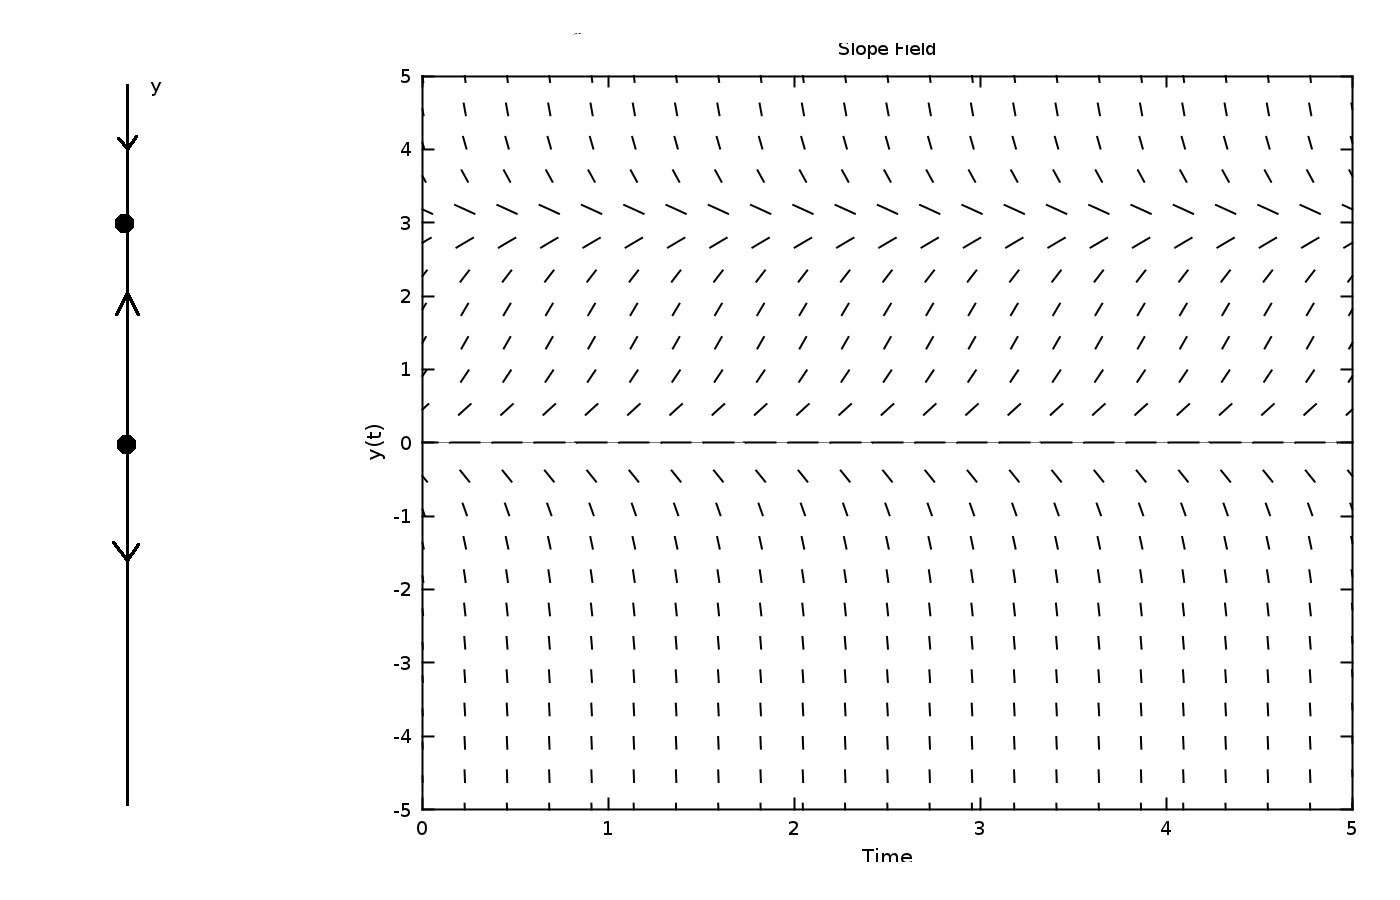
\includegraphics[height=6cm]{img/week3PhaseLineExample1}

\end{frame}


\begin{frame}
  \frametitle{Examples}
  
  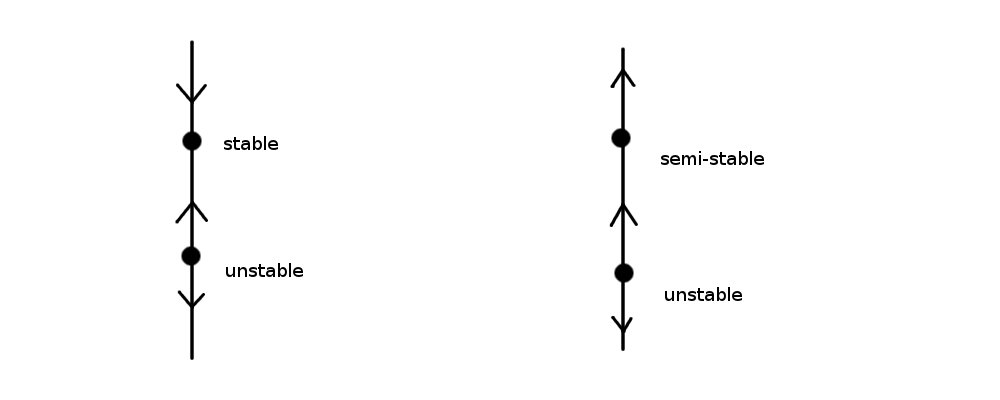
\includegraphics[height=6cm]{img/week3PhaseLine}

\end{frame}

\begin{frame}
  \frametitle{Examples}


  \begin{eqnarray*}
    y' & = & y(2-y)(4-y), \\
    \Rightarrow f(y) & = & y(2-y)(4-y)
  \end{eqnarray*}

  \begin{eqnarray*}
    y' & = & y(2-y^2), \\
    \Rightarrow f(y) & = & y(2-y^2)
  \end{eqnarray*}

  (phase lines drawn on board)

\end{frame}

\iftoggle{clicker}{%
\begin{frame}
  \frametitle{Clicker Quiz}
    
      \ifnum\value{clickerQuiz}=1{%

        Which phase line is the correct phase line for the
        differential equation
        \begin{eqnarray*}
          y ' & = & y^3-y^2
        \end{eqnarray*}

          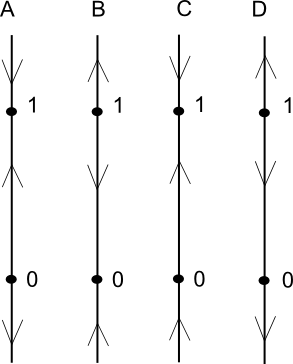
\includegraphics[height=5cm]{img/phaseLinesClickerSect1}

     }\fi

     \ifnum\value{clickerQuiz}=2{%


        Which phase line is the correct phase line for the
        differential equation
        \begin{eqnarray*}
          y ' & = & y^2 + 3y - 4
        \end{eqnarray*}

        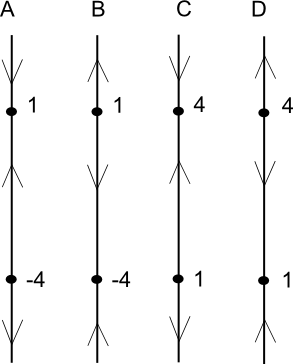
\includegraphics[height=5cm]{img/phaseLinesClickerSect2}


     }\fi

      \ifnum\value{clickerQuiz}=3{%
       Which phase line is the correct phase line for the
        differential equation
        \begin{eqnarray*}
          y ' & = & y^3-y^2
        \end{eqnarray*}

          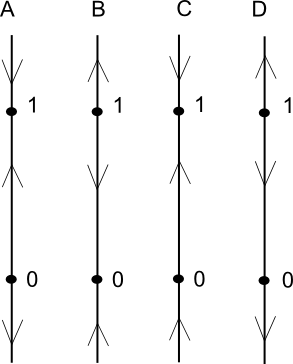
\includegraphics[height=5cm]{img/phaseLinesClickerSect1}
     }\fi

    \vfill
    \vfill
    \vfill

\end{frame}

}



\subsection{Logistic Growth}

\begin{frame}
  \frametitle{Logistic Growth}

  \vspace*{-4em}
  \begin{eqnarray*}
    y' & = & ky,
  \end{eqnarray*}
  
  If $y$ is ``small'' $k$ should be positive.

  If $y$ is ``big'' $k$ should be negative.

  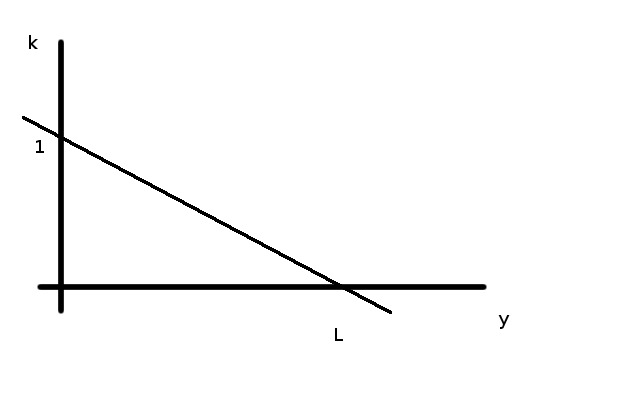
\includegraphics[height=4cm]{img/week3GrowthRate}

  Let 
  \begin{eqnarray*}
    k & = & r \lp 1 - \frac{y}{L} \rp
  \end{eqnarray*}


\end{frame}


\begin{frame}
  \frametitle{Logistic Equation}

  \begin{eqnarray*}
    y' & = & r \lp 1 - \frac{y}{L} \rp y
  \end{eqnarray*}

  Stationary points: $y=0$ and $y=L$. 

  ($L$ is called the ``carrying capacity'')

  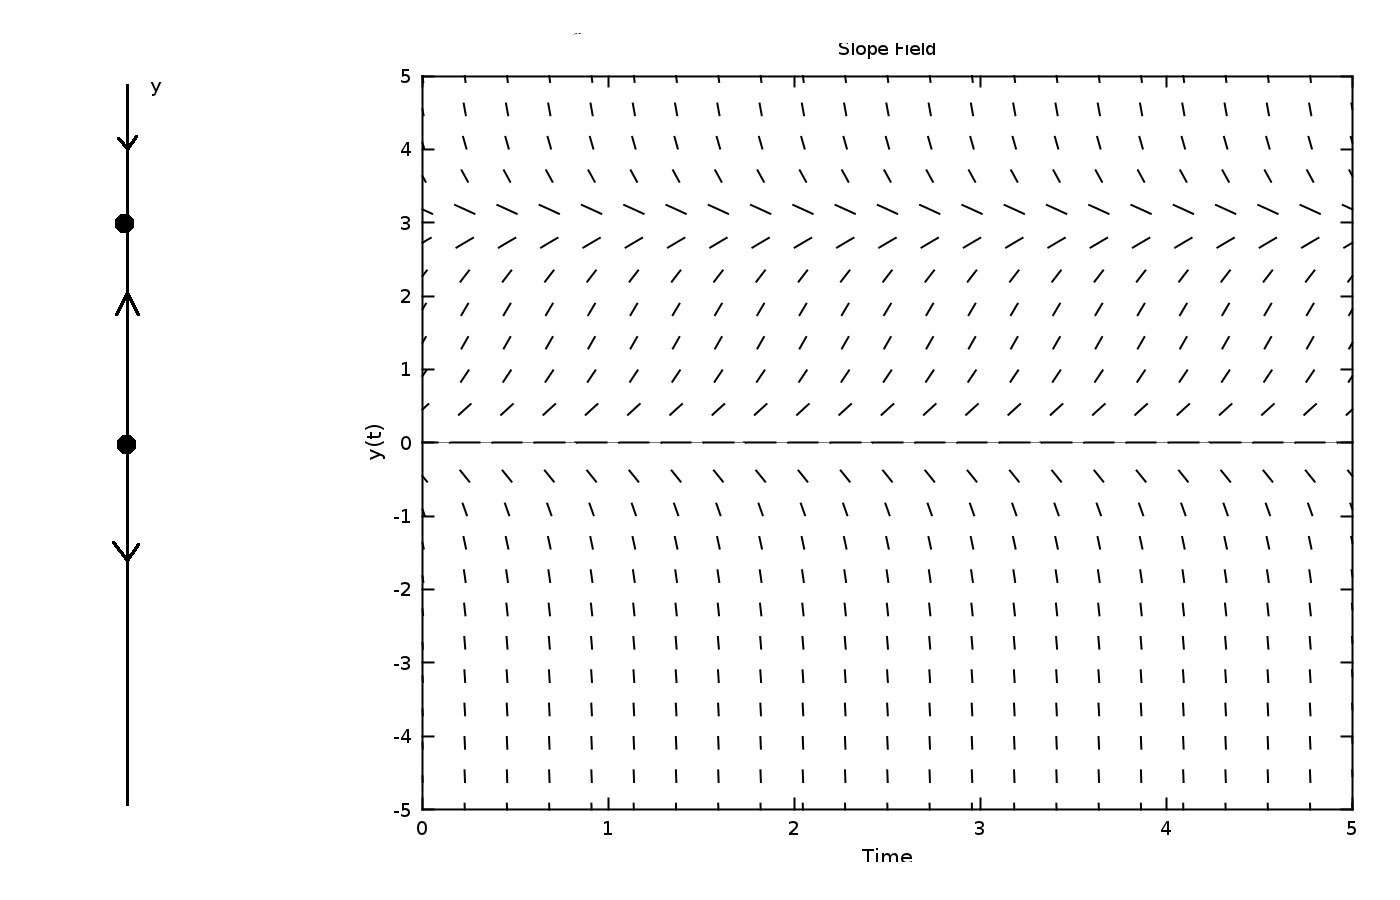
\includegraphics[height=6cm]{img/week3PhaseLineExample1}

\end{frame}


\begin{frame}
  \frametitle{Analytic Solution}

  \begin{eqnarray*}
    y' & = & r \lp 1 - \frac{y}{L} \rp y, \\
    \uncover<2->{
      \frac{y'}{\lp 1 - \frac{y}{L} \rp y} & = & r \\
      \int \frac{y'}{\lp 1 - \frac{y}{L} \rp y} ~ dt & = & \int r ~ dt       
    }
  \end{eqnarray*}

\end{frame}


\begin{frame}


  \begin{eqnarray*}
    \frac{1}{\lp 1 - \frac{y}{L} \rp y} & = & \frac{a}{1 - \frac{y}{L}} + \frac{b}{y} \\
    \Rightarrow 1 & = & a y + b \lp 1 - \frac{y}{L} \rp \\
    b & = & 1, \\
    a & = & \frac{1}{L}
  \end{eqnarray*}

    
\end{frame}

  \begin{frame}

  \begin{eqnarray*}
      \int \frac{1}{\lp 1 - \frac{y}{L} \rp y} ~ dy & = & \int r ~ dt \\
      \int \frac{1}{L} \cdot \frac{1}{1 - \frac{y}{L}} + \frac{1}{y} ~ dy & = & \int r ~ dt \\
      -\ln\lp 1 - \frac{y}{L}\rp + \ln(y) & = & rt + C \\
      \ln\lp\frac{y}{1 - \frac{y}{L}}\rp & = & rt + C \\
      \frac{y}{1 - \frac{y}{L}} & = & k e^{rt} \\
      \Rightarrow y & = & \frac{k e^{rt}}{1 + \frac{k}{L} k e^{rt}}  
  \end{eqnarray*}


  From the initial condition,
  \begin{eqnarray*}
    y(0) & = & y_0, \\
    k & = & \frac{y_0}{1 - \frac{y_0}{L}}
  \end{eqnarray*}
  

\end{frame}

\begin{frame}{Project}

  \begin{tabular}{rclcl}
    rate of change & $=$ & rate in & $-$ & rate out.
  \end{tabular}

  \uncover<2->{

    \vfill 

    We look at the population of fish in an area. Modeling
    assumptions: 

    \vfill

    \begin{tabular}{ll}
      Small population: & linear grown rate. \\
      Large population: & Quadratic death rate.
    \end{tabular}

    \vfill
    This is another way to think about the logistic equation!
    }
  
\end{frame}


\begin{frame}{The terms:}

  \begin{tabular}{ll}
    Population: & $x(t)$ \\
    Parameter:  & A constant value that will be defined later.
  \end{tabular}
  
\end{frame}


\begin{frame}{The Model}

  \begin{eqnarray*}
    \dfrac{dx}{dt} =  bx(t) - (m+cx(t))x(t) - sx(t),
  \end{eqnarray*}
  where we assume that $r = b-m$ is a positive number.

  \vfill

  Here we include one other term, a harvest function, $h(t) = s x(t)$. The
  idea is that the harvest is proportional to how many fish are
  present.
 
\end{frame}

\begin{frame}{Goals}

  \begin{enumerate}
  \item Take part in a meaningful writing exercise!
  \item Your write up should include the following:
    \begin{itemize}
    \item Motivate the model itself and justify the choices made.
    \item Determine the long term behavior of the solution to the
      differential equation.
    \item Determine the stability characteristics of the solution to the
      equation. 
    \item Provide a recommendation for the best value of the harvest
      parameter, $s$, and justify your recommendation.
    \item Determine the solution to the equation and determine if it
      satisfies the predicted behaviors given above.
    \end{itemize}
  \end{enumerate}
  
\end{frame}

\begin{frame}{Plagiarism}

  \redText{You are expected to submit your own work for this project.}
  If you make use of an idea from another source you are expected to
  provide a citation. If you copy the words from another source you
  are expected to put them in quotes and provide a citation. If you
  make use of a figure or diagram from another source you are expected
  to provide a citation. To do otherwise is plagiarism.

  \vfill

  \redText{Any submission found to plagiarize another work will
    receive a zero.}

  \vfill

  You can and are expected to consult written sources or sources on
  the web. Consultation of any living person is limited to an
  instructor for this course, a teaching assistant for this course, or
  your partners. You are expected to consult with the faculty and
  staff at the writing center, but that should be limited to the
  structure of your submission and the writing found in your paper.

\end{frame}

\begin{frame}{Read the Description!}

  It is on moodle.

  Read it for the details. We will use when grading for the
  guidelines.
  
\end{frame}

% LocalWords:  Clarkson pausesection hideothersubsections
